\chapter{Stand van zaken}
\label{ch:stand-van-zaken}
% Tip: Begin elk hoofdstuk met een paragraaf inleiding die beschrijft hoe
% dit hoofdstuk past binnen het geheel van de bachelorproef. Geef in het
% bijzonder aan wat de link is met het vorige en volgende hoofdstuk.

% Pas na deze inleidende paragraaf komt de eerste sectiehoofding.
Niet alles wat in dit onderzoek al is aangekaart, is gemakkelijk te begrijpen. Want natuurlijk zijn de begrippen zoals \emph{Kafka} en \emph{RabbitMq} niet voor iedereen even duidelijk. Ook de term microservices zal bij sommigen de wenkbrauwen wel eens doen fronsen. In dit hoofdstuk is de bedoeling uit te leggen wat al deze begrippen betekenen. Elke tussentitel zal op zijn beurt uitleggen wat een begrip nu eigenlijk is. Na dit hoofdstuk zul je in staat zijn om met deze informatie te begrijpen wat er allemaal gebeurd in dit onderzoek.
\section{Microservices}

Microservices is een software architectuur. De applicatie bestaat uit meerdere kleinere componenten die samen één groot geheel vormen. Deze kleinere componenten zijn onafhankelijk van elkaar en hebben elk hun eigen proces. Deze software architectuur is vrij recent en is de laatste jaren een echte hype aan het worden.

Een belangrijke vraag is: waarom zijn microservices ontstaan? Server-side applicaties gebruiken meestel object-georiënteerde programmeer talen. Deze programmeertalen hebben abstracties om de complexiteit van hun programma's te behandelen in modules. Dit wordt ook wel eens `the monolith` genoemd. Dit is één groot geheel die meestal uit drie lagen bestaat. De presentatielaag, de businesslaag en de datalaag. Deze lagen kunnen niet apart van elkaar gebruikt worden omdat ze verschillende resources met elkaar delen. Dit zorgt ervoor dat bij iedere wijziging in de applicatie, alle lagen opnieuw gereleased worden in een nieuwere versie. Je kan natuurlijk al raden dat dit in een grote applicatie niet de beste oplossing is. 

\begin{figure}[h!]
    \centering
    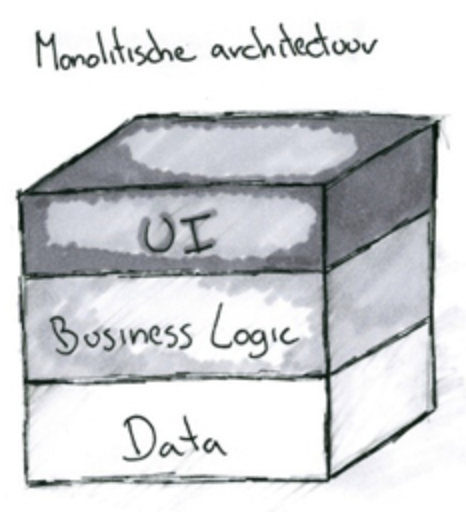
\includegraphics[width=80mm]{../monolith.png}
    \caption{Monolitische architectuur}
        
\end{figure}

Daarom is er een andere architectuur die een heel andere aanpak heeft, namelijk microservices. Dit bestaat uit verschillende kleinere componenten die indien nodig onafhankelijk van elkaar uitgevoerd kunnen worden. Bij deze aanpak is ook belangrijk dat je uw services klein houdt. Hierdoor kunnen je services gemakkelijk hergebruikt, begrepen en opnieuw gebuild worden. Iedere microservice heeft dus maar 1 verantwoordelijkheid.

Omdat microservices op verschillende machines moeten kunnen draaien, bijvoorbeeld op verschillende besturingssystemen, is het beter om ze in te pakken samen met hun dependencies in een container. \emph{Docker} is een voorbeeld van een technologie die deze containers aanbiedt. Door microservices in containers te plaatsen, zorg je ervoor dat de uitvoering van deze services onafhankelijk gebeurd met andere applicaties op dezelfde machine. Containers zijn dus onafhankelijk van een besturingssysteem, hierdoor kunnen microservices op verschillende locaties gedraaid worden. Een van de voordelen hiervan is dat ze door containers in de cloud kunnen geprogrammeerd worden.

De vier grootste voordelen van microservices zijn: 
\begin{itemize}
    \item Schaalbaarheid
    \item Beperken complexiteit
    \item Verkorten time-to-market
    \item Autonomie van ontwikkelteams.
\end{itemize}



 \autocite{Claudio2017} en \autocite{Velthoven2016}



Dit hoofdstuk bevat je literatuurstudie. De inhoud gaat verder op de inleiding, maar zal het onderwerp van de bachelorproef *diepgaand* uitspitten. De bedoeling is dat de lezer na lezing van dit hoofdstuk helemaal op de hoogte is van de huidige stand van zaken (state-of-the-art) in het onderzoeksdomein. Iemand die niet vertrouwd is met het onderwerp, weet er nu voldoende om de rest van het verhaal te kunnen volgen, zonder dat die er nog andere informatie moet over opzoeken \autocite{Pollefliet2011}.

Je verwijst bij elke bewering die je doet, vakterm die je introduceert, enz. naar je bronnen. In \LaTeX{} kan dat met het commando \texttt{$\backslash${textcite\{\}}} of \texttt{$\backslash${autocite\{\}}}. Als argument van het commando geef je de ``sleutel'' van een ``record'' in een bibliografische databank in het Bib\TeX{}-formaat (een tekstbestand). Als je expliciet naar de auteur verwijst in de zin, gebruik je \texttt{$\backslash${}textcite\{\}}.
Soms wil je de auteur niet expliciet vernoemen, dan gebruik je \texttt{$\backslash${}autocite\{\}}. In de volgende paragraaf een voorbeeld van elk.

\textcite{Knuth1998} schreef een van de standaardwerken over sorteer- en zoekalgoritmen. Experten zijn het erover eens dat cloud computing een interessante opportuniteit vormen, zowel voor gebruikers als voor dienstverleners op vlak van informatietechnologie~\autocite{Creeger2009}.

\lipsum[7-20]
